\chapter{Resultat}
Det är kapitlet kommer att beskriva resultatet av den mjukvaran som har utvecklats samt vilka erfarenheter som
teamet har samlat på sig under projektets gång.

\section{Systembeskrivning}
Systemet som skapats består av två separata delar, en back-end och en front-end.

\subsection{Front-end}
Projektets front-end utvecklades i ramverket Angular. Front-end använder sig därför av den komponentbaserade arkitektur som starkt förordas av ramverket. Systemets front-end använder Angulars arkitektur för att implementera designmönstret MVC (se \ref{mvc-ref}).

Det grafiska innehållet på projektets front-end är uppdelat i komponenter som uppdateras eller byts ut till andra komponenter när användaren interagerar med systemet. De komponenter som finns överst i applikationens komponenthierarki är tomma behållare vars enda syfte är att separera applikationens olika beståndsdelar från varandra. Inuti dessa har sedan komponenter med faktiska funktioner, som knappsatser eller sökrutor, placerats.

Applikationen består av flera olika vyer, där vissa av vyerna ska visas upp i samma behållare men vid olika tillfällen, beroende på vilken vy användaren för stunden är intresserad av. För att byta mellan vyerna används Angulars tjänster. Tjänsterna är inte direkt kopplade till någon specifik komponent och används därför för att kommunicera mellan komponenter i olika delar av komponenthierarkin.

All den data om patienter, salar och utrustning som användaren är intresserad av finns på en server i projektets back-end. Därför är det nödvändigt med kommunikation mellan de båda delarna. På projektets front-end sköts kommunikationen med AJAX-anrop. Dessa anrop sker i tjänster för att de ska vara tillgängliga för alla komponenter som behövde tillgång till data av olika sorter.

\subsection{Back-end}
Back-end i projektet är en server som har två huvuduppgifter. Den första är att vara värd för klienten så att den kan kommas åt av flera användare och datorer över nätverk. Den andra uppgiften är att ha en databas med tillhörande webb-API. Databasen används för att hantera all data som behövs för schemaläggningen som bland annat operationsbeslut, kirurger, resurser och bokningar med mera. Webb-API tillåter klienten att kunna logga in och sedan hämta och modifiera denna data.

Servern är byggd på miljön Node.js och är skriven i JavaScript. Den använder sig av Node.js-biblioteket Express för den statiska leveransen och klienten och för att definiera HTTP-API:t. För hantering av databasen används i grunden MySQL men även ORM-biblioteket Sequelize i Node.js. Sequelize tillåter objekt-orienterad hantering av databasen och tar bort behovet att använda direkta SQL-frågor. All test-data som används i prototypen läggs också in i databasen med hjälp av seeds i Sequelize. Mer om seeds och Sequelize går att läsa i stycke \ref{sequelize_teori} i teorin.

Hela API:et i servern skyddas bakom autensiering. Detta görs med hjälp av Node.js-biblioteket Passport och ser till att ingen data i databasen kan kommas åt eller modifieras utan att först logga in.

\subsection{LoFi-Prototyper}

\begin{figure}[H]
  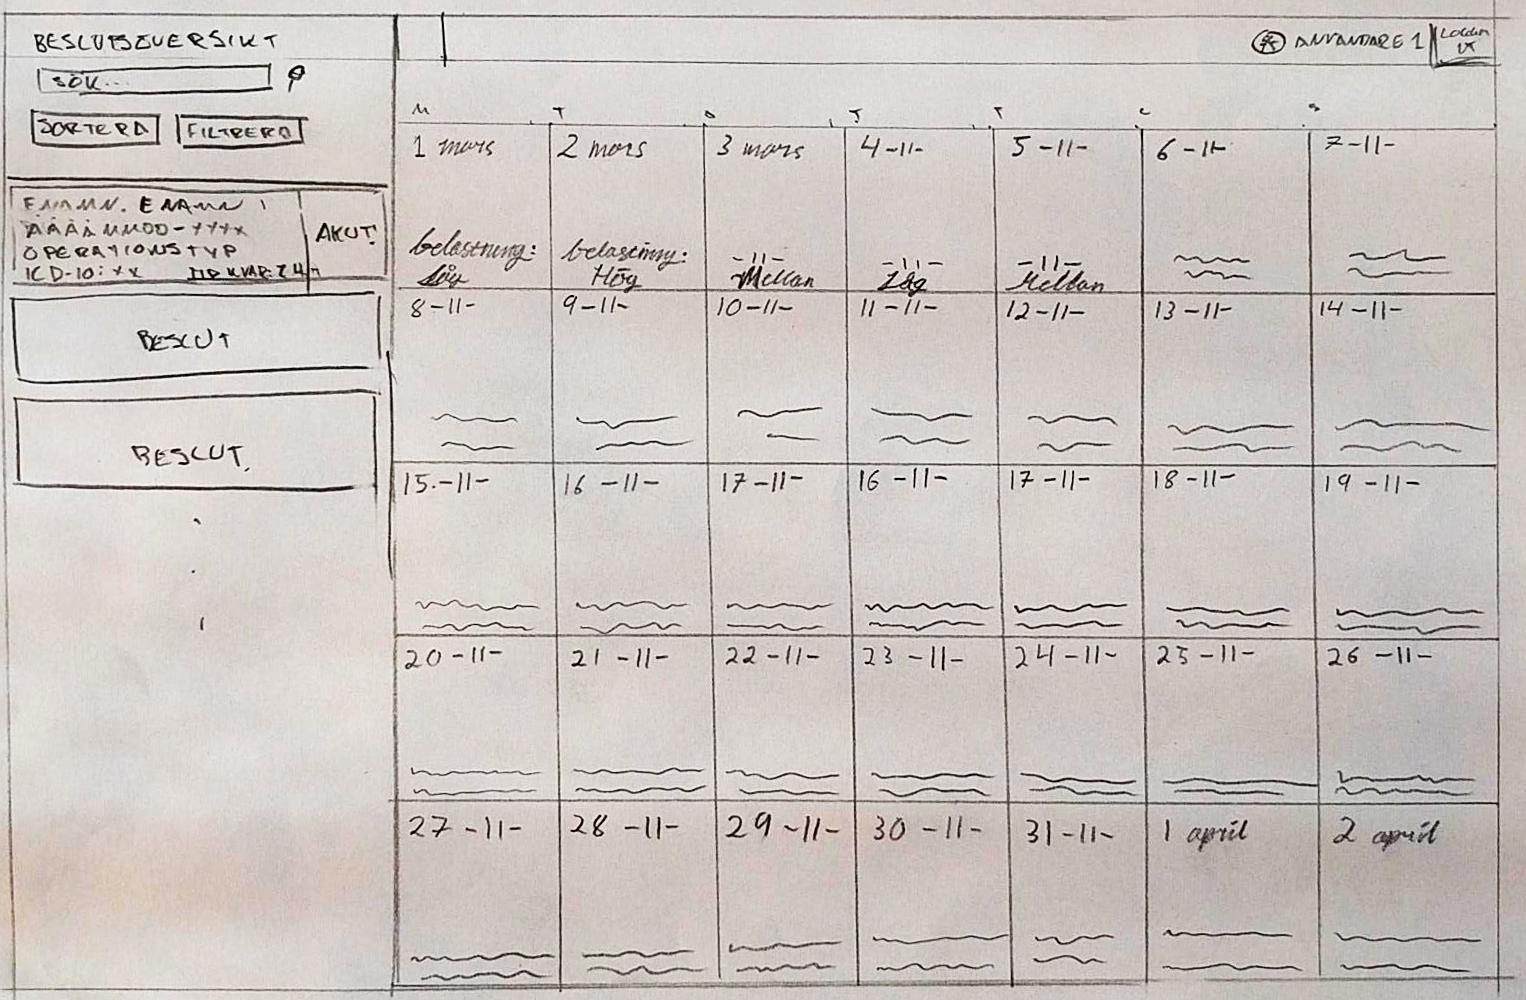
\includegraphics[width=\linewidth]{Figures/LoFi_no2.jpg}
  \caption{Sista LoFi-prototypen}
  \label{fig:LofiPic}
\end{figure}


Under projektets andra iteration utvecklades tre olika LoFi-prototyper. Dessa
LoFi-prototyper designades för att visa på olika designalternativ på
användargränssnittet. Ett exempel på detta är informationen som var med i listan
över beslutade operationer.

I en av prototyperna identifierades patienten som hörde ihop med beslutet med namn, den andra med personnummer. I den tredje LoFi-prototypen
fanns inget som identifierade patienten utan enbart information om vilken
typ av operation det var. På liknande sätt utvärderades olika sätt att
visualisera lediga tider i schemat samt olika sätt att anpassa sökparametrarna för en sökning efter lediga tider.

När prototyperna visades för kunden kunde alternativen sållas bort och en tydligare bild av behoven framträdde.
Till exempel fanns det endast personnummer och inte namn på patienterna, vilket var något som önskades.

Den första iterationen av LoFi-prototyper användes sedan för att ta fram en ny
LoFi-prototyp, som uppdaterats enligt återkoppling från föregående iteration. Den nya LoFi-prototypen visades för tre olika operationsplanerare för att få deras tankar och idéer om den grafiska designen. (Figur \ref{fig:LofiPic} illustrerar en bild av den sista Lofi-prototypen.)

\subsection{Systemanatomi}
I första iterationen togs det fram en systemanatomi (se figur \ref{fig:Systemanatomi}) som användes under projektets gång som ett hjälpmedel för strukturera upp arbetet under utvecklingen. Den gav en översiktlig bild av vilken funktionalitet produkten skulle innehålla och hur de olika delarna samverkade med varandra. Utöver detta presenterades den i ett tidigt skede för kunden i syfte att säkerställa att projektgruppens syn på systemet stämde överens med kundens.

\begin{figure}[H]
    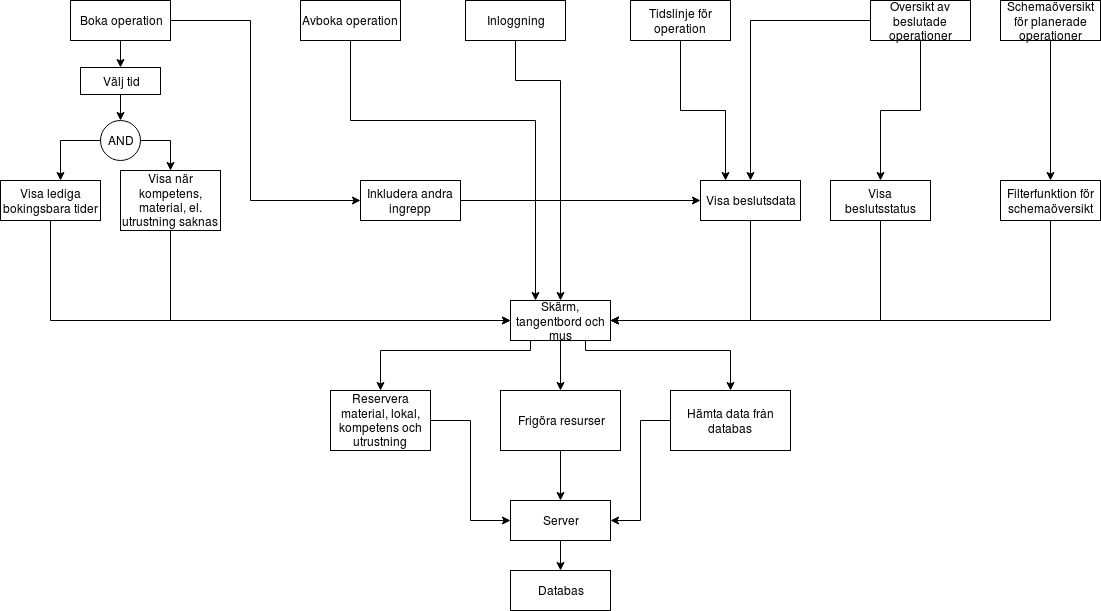
\includegraphics[width=\textwidth,height=.4\textheight]{Figures/Systemanatomi.png}\\
    \caption{Systemanatomi}
    \label{fig:Systemanatomi}
\end{figure}

\subsection{Värde för kund}
Den produkt som har skapats är ett lättöverskådligt schemaläggningssystem för operationer. Slutprodukten tillsammans med tankar och erfarenheter från design och utvecklings-faserna kommer att ha ett stort värde för kunden. Detta eftersom projektet kommer att användas som en form av förstudie till ett större projekt (se stycke \ref{sec:syfte}).

Det medför att Region Östergötland kommer att ha något att utgå ifrån då deras projekt startar, vilket hjälper av flera anledningar. Projektägaren som också är insatt i det större projektet kommer att kunna ta med sig många erfarenheter från det här projekt.

\section{Gemensamma erfarenheter}
I början av projektet fick vi snabbt större erfarenhet av olika områden
tack vare de olika presentationer som de olika deltagarna i projektet gav.
Vi fick även en ökad förståelse för hur delar av sjukvården fungerar och att ett bra
it-system kan göra verklig skillnad.

\section{Översikt över individuella bidrag}
I denna delen presenteras deltagarnas individuella bidrag översiktligt.

\todo{Lägg till era rubriker och en kort synopsis här}
\subsection{Adam}
En studie i hur teamledarens roll går att applicera tillsammans med scrum-metodik.
\subsection{Björn}
Hur kan versionshantering användas effektivt för ett mindre mjukvaruutvecklings projekt.
\subsection{Christoffer}
Betydelsen av att samla krav från en varierad grupp aktörer
\subsection{Henrik}
För/nackdelar med TypeScript jämfört med JavaScript
\subsection{Martin}
Angular som webbutvecklingsplattform
\subsection{Niclas}
Prototypuveckling i kandidatprojekt
\subsection{Tor}
Kvalitetsförsäkrande metoder i ett småskaligt mjukvaruprojekt
